\documentclass{article}
\usepackage[rightcaption]{sidecap}
\usepackage{graphicx} % Required for inserting images
\usepackage{multirow}
\usepackage[top=4cm, bottom=4cm, left=3cm, right=3cm]{geometry}
\usepackage[labelfont=bf, justification=raggedright, singlelinecheck=false]{caption}
\usepackage[european, americanvoltages]{circuitikz} % Per i circuiti
\usepackage{pgfplots}
\pgfplotsset{compat=1.18} % Ottimizza la compatibilità di PGFPlots
\usepgfplotslibrary{groupplots} % Consente di allineare modulo e fase
\newcommand\tab[1][1cm]{\hspace*{#1}}
\usepackage[T1]{fontenc}
\usepackage{appendix}
\usepackage{tabularx}
\usepackage{float}
\usepackage{tcolorbox}
\usepackage{amsmath}
\usepackage{amssymb}
\usepackage{eso-pic} % for \BgThispage
\usepackage{tikz}
\usepackage{titlesec}
\usepackage{tocloft}
\usetikzlibrary{arrows.meta}
\usepackage[pages=some]{background}
\usepackage[italian]{babel}
\usepackage[colorlinks=true, linkcolor=black, citecolor=black, filecolor=black, urlcolor=blue]{hyperref}
\addto\captionsitalian{\renewcommand{\contentsname}{Indice}}
\backgroundsetup{scale=1.5,anchor=right,angle=0,opacity=0.1,contents={
\includegraphics[scale=1]{Misc/logo_standard (1).png}}}

% FORMATTAZIONE SOTTOTITOLI
%-----------------------------------------------------------
\titleformat{\subsection}
{\normalfont\Large\bfseries}{\thesubsection}{1em}{}

\titleformat{\section}
{\normalfont\Large\bfseries}{\thesection}{1em}{}
%-----------------------------------------------------------

% FORMATTAZIONE INDICE
%-----------------------------------------------------------
\renewcommand{\cftsecfont}{\normalfont\Large\bfseries}
\renewcommand{\cftsecpagefont}{\normalfont\Large\bfseries}

\renewcommand{\cftsubsecfont}{\normalfont\Large}
\renewcommand{\cftsubsecpagefont}{\normalfont\Large}

\setlength{\cftbeforesecskip}{0.5cm} 
\setlength{\cftbeforesubsecskip}{0.3cm}
%-----------------------------------------------------------

% TITOLO
%-----------------------------------------------------------
\title{
    Relazione : Attuatore Elettro-meccanico e Diodo di Freewheeling \\ 
    \vspace{0.3cm} 
    \Large Gruppo 100
}
%-----------------------------------------------------------

% AUTORI
%-----------------------------------------------------------
\author{
  Lorenzo Allocco \\ -- Mat. 0612709084
  \\ \\
  Riccardo La Porta \\ -- Mat. 0612709691
  \\ \\
  Francesco Grimaldi \\ -- Mat. 0612708839
  \\ \\
  Alessandro Altieri \\ -- Mat. 0612709239
}

\date{13 Giugno 2026}

\begin{document}
\BgThispage

\AddToShipoutPictureBG*{
  \begin{tikzpicture}[remember picture, overlay]
    \node [anchor=north west, inner sep=30pt] at (current page.north west)
      {
\includegraphics[height=1.5cm]{Misc/diem (1).png}};
  \end{tikzpicture}
}
%-----------------------------------------------------------

\maketitle

% INDICE
%-----------------------------------------------------------
\newpage
\tableofcontents
\newpage
%-----------------------------------------------------------

\section{Obiettivi dell'esperienza}
    La seguente relazione si pone come obiettivo quello di descrivere l'esperienza di laboratorio tenutasi
    nell'ambito del corso di Tecnologie Elettriche per l'informatica Industriale.\\

    \noindent In particolare, questa esperienza si è focalizzata sul funzionamento di un magnete solenoide
    pilotato da raspberry tramite transistor BJT e degli effetti induttivi generati dal suo funzionamento. 
    Inoltre, è stato analizzato il ruolo fondamentale del diodo di freewheeling (o di ricircolo) nella protezione
    dei componenti elettronici dalle sovratensioni generate dall'interruzione della corrente in un carico induttivo.

\section{Introduzione e cenni teorici}

    Un carico induttivo è un elemento di circuito caratterizzato dalla capacità di immagazzinare energia sotto forma
    di campo magnetico. La grandezza che descrive questa proprietà è l'induttanza $L$, misurata in henry [H]. La relazione
    fondamentale che governa il comportamento di un induttore è:
    
    \begin{equation}
        \boxed{V_L = L \frac{di}{dt}}
    \end{equation}
    
    \noindent Essa implica che la tensione ai capi dell'induttore è proporzionale alla velocità di variazione della corrente che lo
    attraversa. Ne consegue che ogni volta che si tenta di interrompere bruscamente la corrente in un carico induttivo
    (come accade alla commutazione di un transistor), il termine $di/dt$ assume valori molto elevati, producendo un picco di
    sovratensione (spike) potenzialmente distruttivo per i componenti a semiconduttore del circuito di pilotaggio.

    \subsection{Circuito RL -- transitorio di carica e scarica}
        Un carico induttivo reale è modellabile come una serie di una resistenza $R$ (resistenza interna degli avvolgimenti)
        e un'induttanza $L$. All'accensione del circuito (transistor in conduzione), la corrente segue un andamento esponenziale
        crescente:
        
        \begin{equation}
            \boxed{i(t) = \frac{V_{CC}}{R}\left(1 - e^{-t/\tau}\right), \quad \tau = \frac{L}{R}}
        \end{equation}
        
        \noindent dove $\tau$ è la costante di tempo del circuito RL. Per il solenoide TAU-0730TM impiegato nell'esperienza ($R = 40\,\Omega$,
        $V_{CC} = 12\,\text{V}$), la corrente a regime vale:
        
        \begin{equation*}
            \boxed{I_\infty = \frac{V_{CC}}{R} = \frac{12}{40} = 300\,\text{mA}}
        \end{equation*}
        
        \noindent All'apertura del circuito (transistor in interdizione), in assenza di un percorso alternativo per la corrente, l'energia
        immagazzinata nel campo magnetico $\left(W = \frac{1}{2}LI^2\right)$ deve essere dissipata istantaneamente, generando il picco
        di tensione induttiva descritto dall'equazione (1).
    \newpage
    \subsection{Il transistor BJT come interruttore}
        Il transistor BDX33C è un dispositivo NPN Darlington con tensione collettore-emettitore massima $V_{CEO} = 100\,\text{V}$ e
        corrente di collettore massima $I_C = 10\,\text{A}$. Nel circuito è pilotato in commutazione: un segnale di onda quadra generato
        dal Raspberry Pi viene applicato alla base tramite una resistenza di limitazione da $1\,\text{k}\Omega$, portando il transistor
        in saturazione (ON) o in interdizione (OFF). Poiché la tensione di breakdown collettore-emettitore è 100 V, lo spike induttivo non
        smorzato potrebbe facilmente superare tale soglia e danneggiare irreversibilmente la giunzione.

    \subsection{Il diodo di freewheeling}
        Il diodo di freewheeling (o diodo di ricircolo) è un diodo collegato in antiparallelo al carico induttivo: il catodo è connesso verso
        il polo positivo dell'alimentazione, l'anodo verso il collettore del transistor. In condizioni normali (transistor ON), il diodo è
        polarizzato inversamente e non conduce. All'apertura del circuito (transistor OFF), il diodo si polarizza in diretta e offre un percorso
        a bassa impedenza per la corrente induttiva residua, limitando la tensione ai capi del transistor al valore:
        
        \begin{equation}
            \boxed{V_{CE,max} = V_{CC} + V_F}
        \end{equation}
        
        \noindent dove $V_F$ è la tensione di soglia diretta del diodo. L'energia viene quindi dissipata gradualmente attraverso la resistenza interna
        del solenoide e la resistenza dinamica del diodo, con una costante di tempo:
        
        \begin{equation}
            \boxed{\tau' = \frac{L}{R_{solenoide} + R_{diodo}}}
        \end{equation}
        
        \noindent Il diodo FEP16DT scelto per l'esperienza appartiene alla famiglia FEP16xT di Vishay, un raddrizzatore ultrafast a doppio catodo comune in
        package TO-220AB. Le sue caratteristiche principali, ricavate dal datasheet ufficiale, lo rendono particolarmente adatto all'applicazione:
        
        \begin{itemize}
            \item \textbf{Tensione di picco inversa massima} $V_{RRM} = 200\,\text{V}$: ampiamente superiore ai 12 V di alimentazione, garantendo un adeguato margine di sicurezza.
            \item \textbf{Corrente media raddrizzata} $I_{F(AV)} = 16\,\text{A}$ a $T_C = 100\,\text{C}$: ben al di sopra della corrente nominale del solenoide ($\approx 300\,\text{mA}$).
            \item \textbf{Tempo di reverse recovery} $t_{rr} = 50\,\text{ns}$: il recupero ultrarapido minimizza le perdite di commutazione e lo spike di corrente inversa durante la transizione.
            \item \textbf{Tensione di soglia diretta} $V_F = 1{,}30\,\text{V}$ a 8,0 A: applicando l'equazione (3), la tensione massima sull'interruttore risulta $V_{CE,max} \approx 12 + 1{,}30 = 13{,}30\,\text{V}$, ampiamente entro il limite di 100 V del transistor BDX33C.
        \end{itemize}
\newpage


\section{Strumentazione e componenti utilizzati}
    La strumentazione utilizzata durante l'esperienza è elencata nella tabella seguente:

    \begin{table}[H]
        \centering
        \begin{tabularx}{\textwidth}{|X|X|X|}
            \hline
            \textbf{Strumento} & \textbf{Modello} & \textbf{Caratteristiche} \\ \hline
                Oscilloscopio Digitale & Hantek 6022BL & 2 canali, 20 MHz, 48 MS/s \\ \hline
                Software & DPO & Software per macchine Windows \\ \hline
                Software & OpenHantek & Software open source disponibile su macchine linux \\ \hline
        \end{tabularx}
        \caption{Specifiche della strumentazione di laboratorio.}
    \end{table}

    I componenti utilizzati durante l'esperienza sono elencati nella tabella seguente:

    \begin{table}[H]
        \centering
        \begin{tabularx}{\textwidth}{|X|X|X|}
            \hline
            \textbf{Componente} & \textbf{Modello} & \textbf{Caratteristiche} \\ \hline
            Elettromagnete Solenoide & TAU-0730TM & 12V DC, $40\Omega$, 0.5N spinta,   \\ \hline
            Diodo & FEP16DT & 200V, 16A\\ \hline
            Transistor BJT & BDX33C& NPN Darlington, 100V, 10A \\ \hline
            Resistore&  Resistore & 1K$\Omega$ \\ \hline
        \end{tabularx}
        \caption{Componenti utilizzati.}
    \end{table}

    \begin{figure}[H]
        \centering
        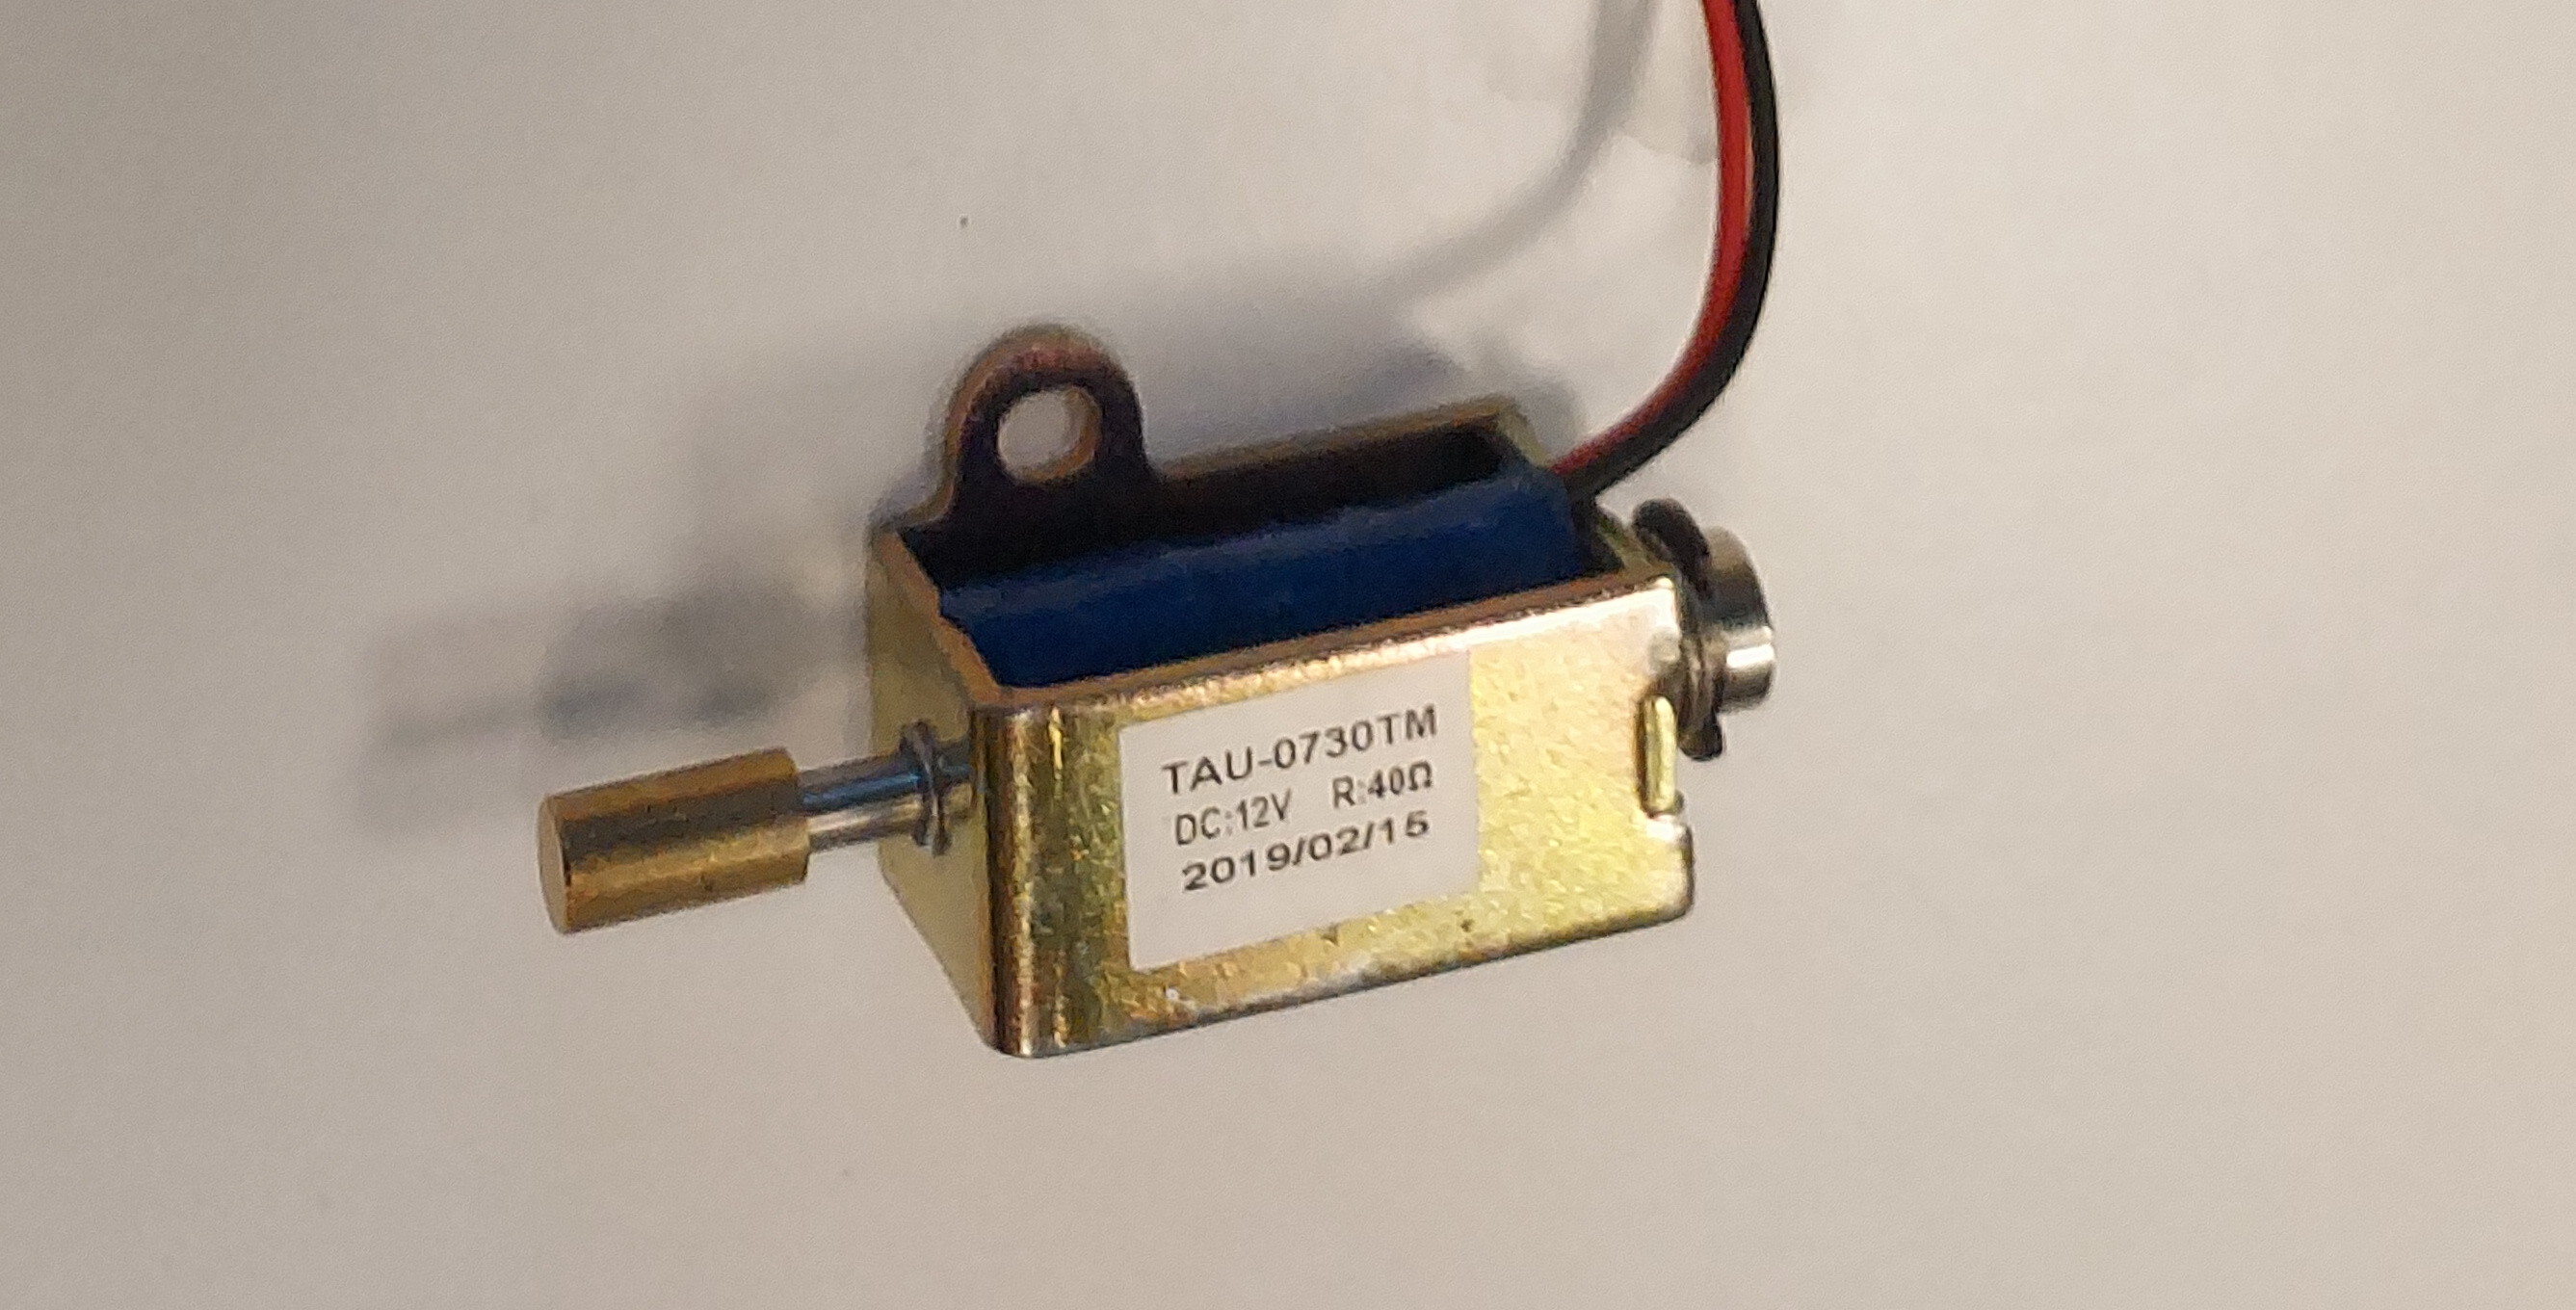
\includegraphics[width=0.6\textwidth]{Misc/attuatore.png}
        \caption{Elettromagnete solenoide TAU-0730TM.}
    \end{figure}

    \begin{figure}[H]
        \centering
        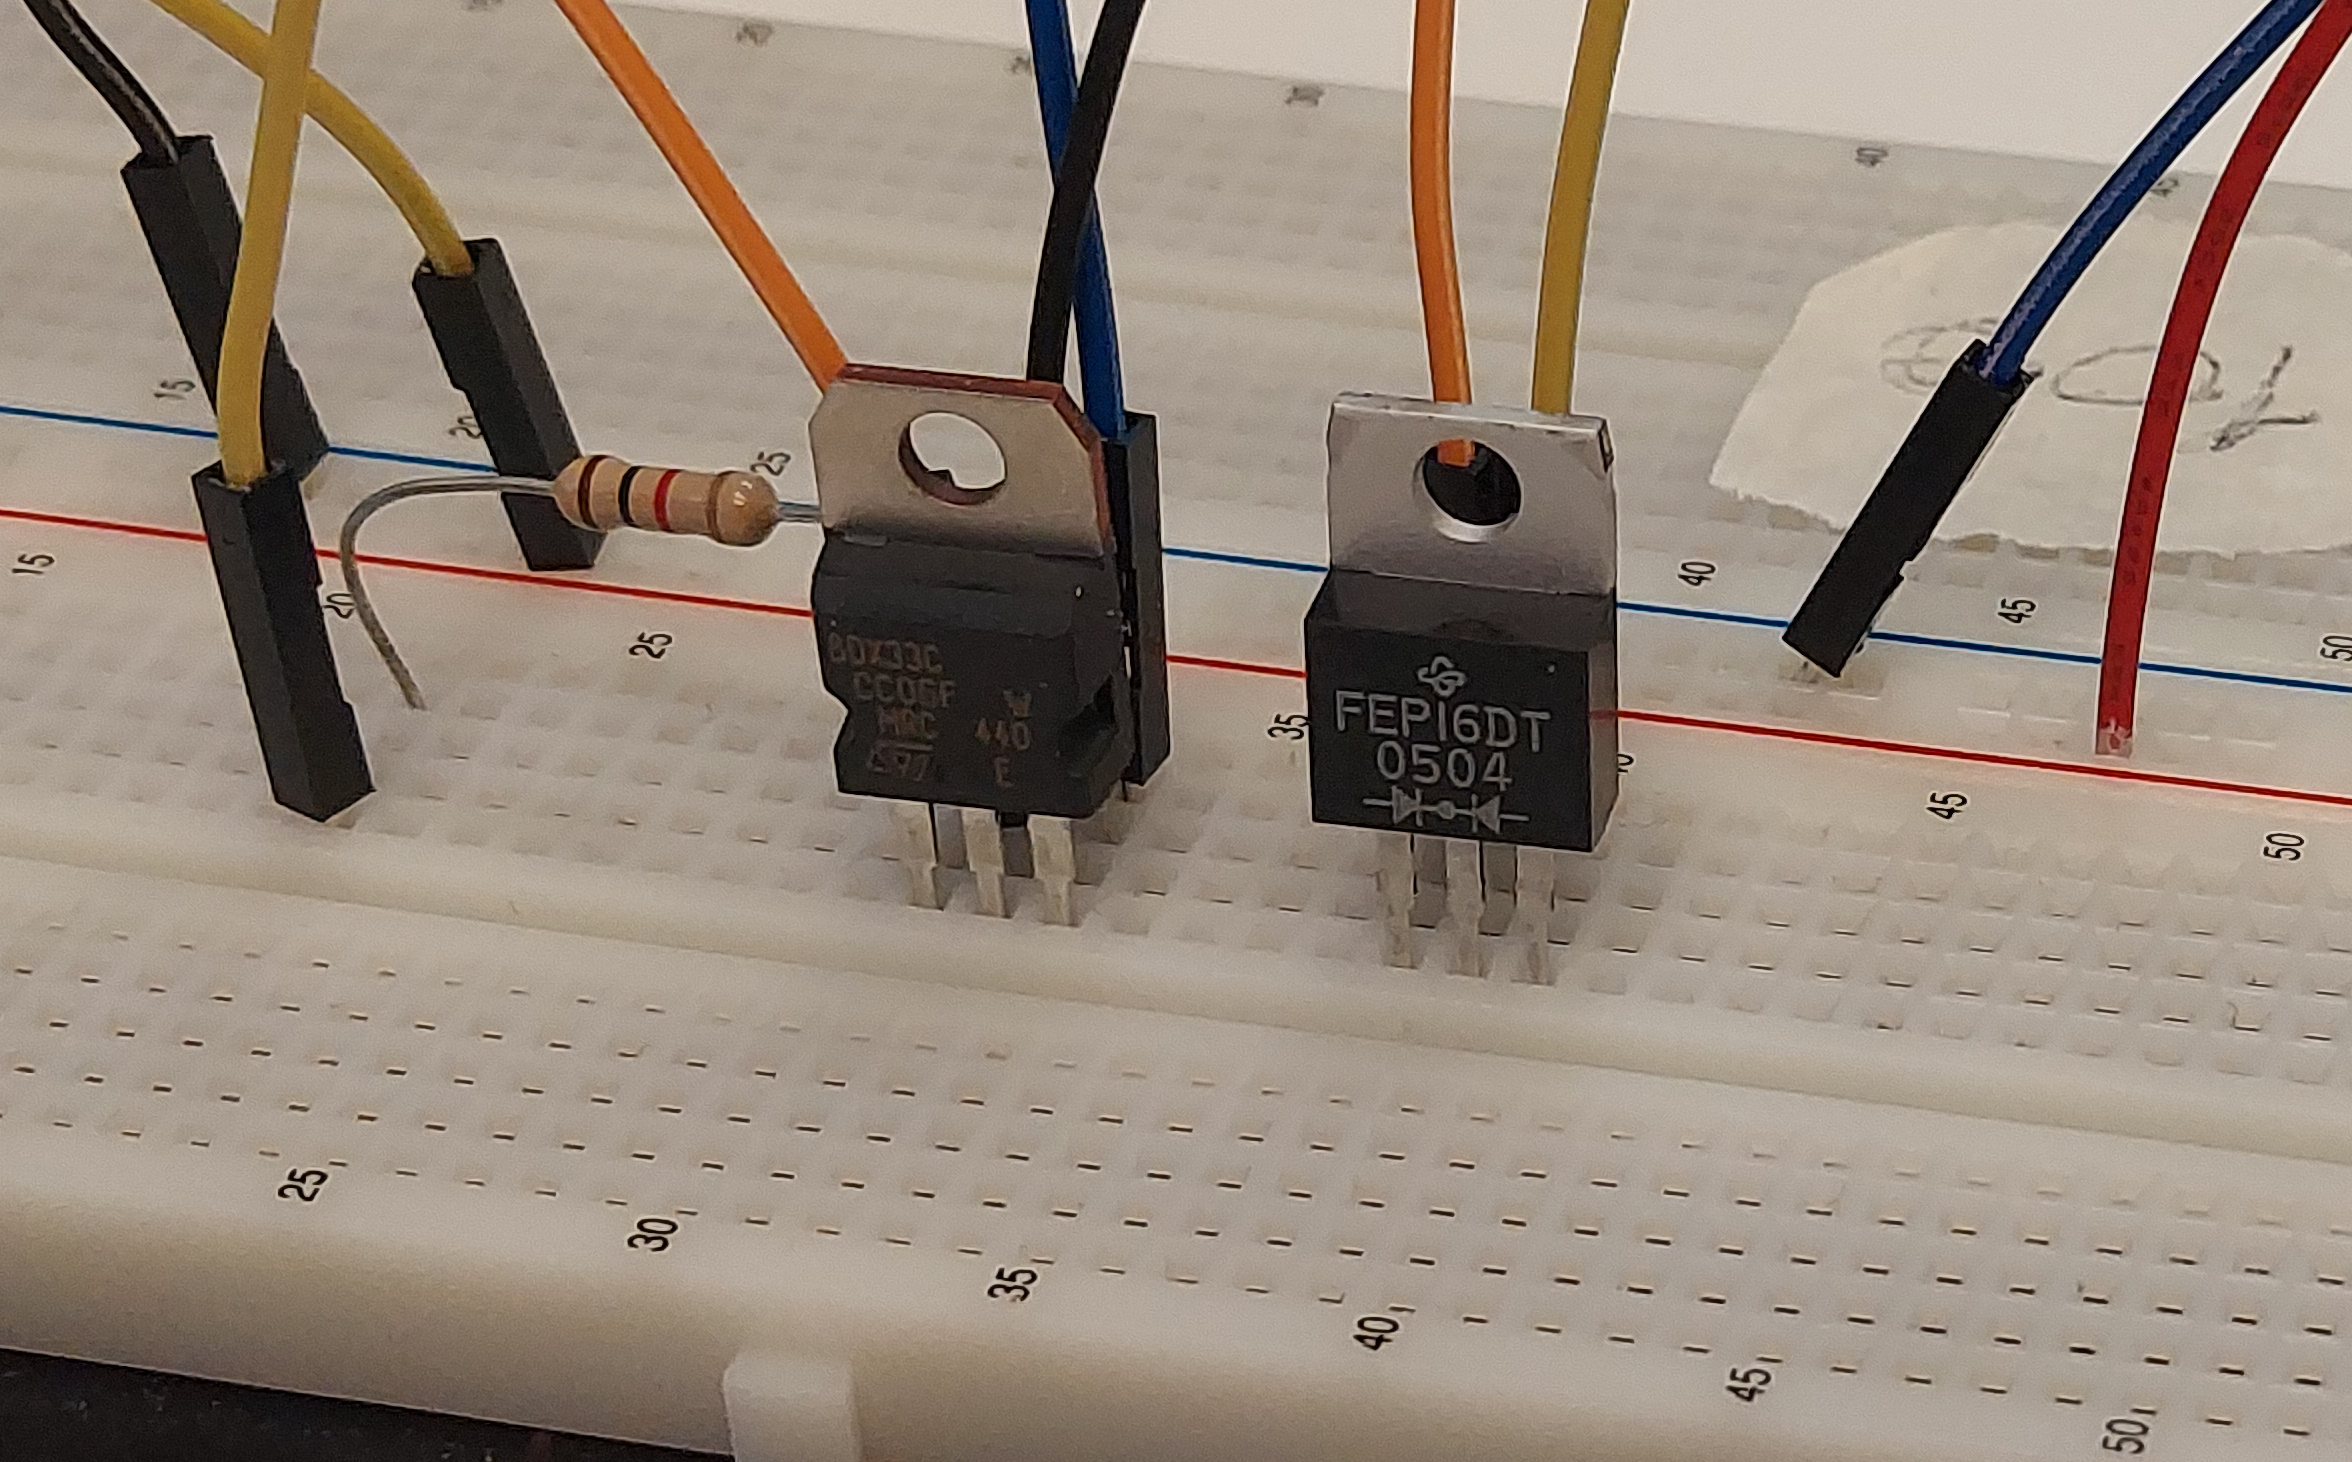
\includegraphics[width=0.6\textwidth]{Misc/dettaglio_componenti.jpg}
        \caption{Da sinistra : resistore 1K$\Omega$, transistor BDX33C, diodo FEP16DT.}
        \label{fig:dettaglio_componenti}
    \end{figure}

\section{Schema del circuito e procedura sperimentale}
    Il circuito realizzato permette di pilotare il solenoide attraverso un transistor BJT NPN.
    Il segnale di comando viene inviato alla base del transistor, il quale agisce come interruttore
    per far fluire corrente attraverso il carico induttivo. Successivamente, in parallelo al solenoide,
    viene inserito il diodo di freewheeling connesso in polarizzazione inversa rispetto all'alimentazione principale.

    \subsection{Circuito di pilotaggio base} 
     Viene assemblato il circuito base senza diodo di protezione. Le sonde dell'oscilloscopio vengono collegate per monitorare l'onda quadra in ingresso e la tensione ai capi del solenoide, al fine di evidenziare la differenza, e quindi lo spike di sovratensione induttiva.
    \begin{figure}[H]
        \centering
        \includegraphics[width=0.8\textwidth]{Misc/misura_nodiodo.jpg}
        \caption{Foto del setup sperimentale con i componenti collegati su breadboard.}
        \label{fig:setup_sperimentale_no_diodo}
    \end{figure}

    \newpage

    Lo schema equivalente del circuito risulta:
    \begin{figure}[H]
        \centering
        
            \begin{circuitikz}[american, thick]
                
            
                \node[npn] (Q) at (0,0) {};
                \node[right=2pt] at (Q.C) {C};
                \node[below right=2pt] at (Q.E) {E};
                \node[below=2pt] at (Q.B) {B};

                
                \draw (Q.C) -- (0,1.5) coordinate (c_split);
                \node[circ] at (c_split) {};

            
                \draw (c_split) to[L] (0,3.5) coordinate (c_join);
                \node[circ] at (c_join) {};

                
                \draw (c_join) -- (3,3.5) to[V, l=+12V] (3,-1.5) coordinate (gnd_right);
                
                
                \draw (Q.E) -- (0,-1.5) coordinate (gnd_mid);
                \node[circ] at (gnd_mid) {};
                \draw (gnd_right) -- (gnd_mid);

                
                \draw (Q.B) to[R, l=1k$\Omega$] (-3,0) coordinate (sig_in);
                
                
                \draw (sig_in) to[sqV] (-3,-1.5) coordinate (gnd_left);
                \draw (gnd_left) -- (gnd_mid);

            \end{circuitikz}
        \caption{Schema del collegamento dei componenti con diodo.}
        \label{fig:schema_collegamento}
    \end{figure}

    \subsection{Circuito con diodo di freewheeling}
    Si integra poi il diodo all'interno del circuito per fornire un percorso di scarica alla corrente. Si effettuano nuovamente le misurazioni per verificare l'eliminazione del picco di tensione inversa durante il transitorio.

    \begin{figure}[H]
        \centering
        \includegraphics[width=0.8\textwidth]{Misc/misura_diodo.jpg}
        \caption{Foto del setup sperimentale con i componenti collegati su breadboard.}
        \label{fig:setup_sperimentale}
    \end{figure}

    \newpage

    Lo schema equivalente aggiornato risulta:
    \begin{figure}[H]
        \centering
        
            \begin{circuitikz}[american, thick]
                
            
                \node[npn] (Q) at (0,0) {};
                \node[right=2pt] at (Q.C) {C};
                \node[below right=2pt] at (Q.E) {E};
                \node[below=2pt] at (Q.B) {B};

                
                \draw (Q.C) -- (0,1.5) coordinate (c_split);
                \node[circ] at (c_split) {};

            
                \draw (c_split) to[L] (0,3.5) coordinate (c_join);
                \node[circ] at (c_join) {};

                \draw (c_split) -- (-1.5,1.5) to[D] (-1.5,3.5) -- (c_join);
                
                \draw (c_join) -- (3,3.5) to[V, l=+12V] (3,-1.5) coordinate (gnd_right);
                
                
                \draw (Q.E) -- (0,-1.5) coordinate (gnd_mid);
                \node[circ] at (gnd_mid) {};
                \draw (gnd_right) -- (gnd_mid);

                
                \draw (Q.B) to[R, l=1k$\Omega$] (-3,0) coordinate (sig_in);
                
                
                \draw (sig_in) to[sqV] (-3,-1.5) coordinate (gnd_left);
                \draw (gnd_left) -- (gnd_mid);

            \end{circuitikz}
        \caption{Schema del collegamento dei componenti con diodo.}
        \label{fig:schema_collegamento_diodo}
    \end{figure}

\section{Raccolta e Analisi dei dati sperimentali}
    In questa fase dell'esperimento sono state effettuate diverse misurazioni per osservare il comportamento del solenoide durante le fasi di
    eccitazione e diseccitazione, con particolare attenzione ai transitori di tensione.

    \subsection{Analisi del transitorio senza diodo di freewheeling}
        Inizialmente è stato configurato il circuito pilotando il solenoide tramite il transistor BJT senza l'ausilio del diodo di protezione.
        All'apertura del circuito (interruzione della corrente nel carico induttivo), l'oscilloscopio ha rilevato un picco di tensione inversa
        molto elevato (sovratensione induttiva). Questo fenomeno è dovuto alla legge di Faraday-Lenz:
        
        \begin{equation}
            \boxed{V_L = L \frac{di}{dt}}
        \end{equation}
        
        \noindent Poiché la variazione di corrente $di$ avviene in un tempo $dt$ estremamente ridotto, la tensione generata tende a valori teoricamente
        infiniti, rischiando di danneggiare la giunzione del transistor.

        \begin{figure}[H]
            \centering
            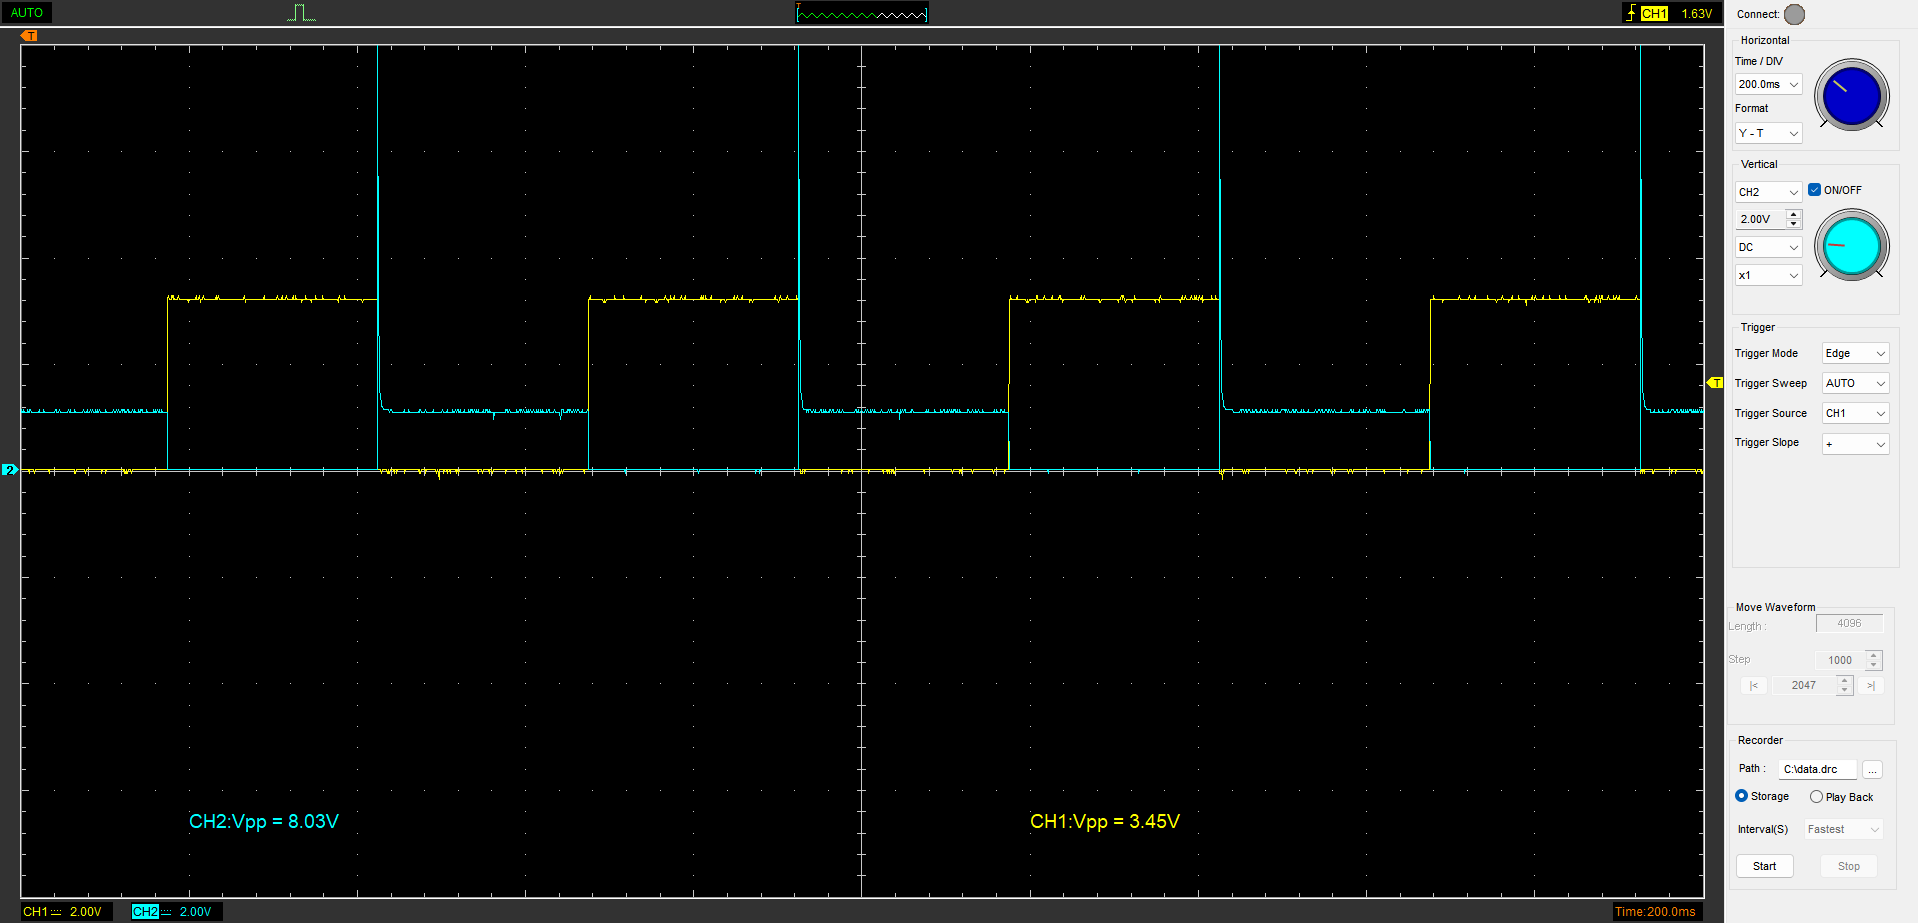
\includegraphics[width=1\textwidth]{Misc/no_diodo.png}
            \caption{Misurazione all'oscilloscopio del transitorio senza diodo di freewheeling.}
            \label{fig:transitorio_senza_diodo}
        \end{figure}

        \noindent Analizzando la traccia acquisita dall'oscilloscopio, riportata in figura \ref{fig:transitorio_senza_diodo}, si osserva in giallo il
        segnale utilizzato per il pilotaggio del transistor. In azzurro è invece rappresentata la tensione ai capi del solenoide, in cui risulta
        evidente il picco (spike) di sovratensione induttiva che si genera all'istante di apertura del circuito.

    \subsection{Analisi del transitorio con diodo di freewheeling}
        Successivamente è stato inserito il diodo in parallelo al solenoide, con il catodo rivolto verso l'alimentazione positiva. In questa configurazione,
        nel momento in cui il transistor smette di condurre, il diodo entra in conduzione diretta offrendo un cammino a bassa impedenza per la corrente
        accumulata nell'induttore. Le osservazioni effettuate mostrano che:

        \begin{itemize}
            \item La tensione ai capi del transistor viene limitata a $V_{CC} + V_F$ (dove $V_F$ è la tensione di soglia del diodo).
            \item L'energia immagazzinata nel campo magnetico viene dissipata gradualmente attraverso la resistenza interna del solenoide e del diodo stesso.
            \item Il tempo di rilascio meccanico dell'attuatore risulta leggermente superiore rispetto al caso senza diodo, a causa del prolungamento della
                  circolazione di corrente determinato dalla costante di tempo $\tau = \frac{L}{R_{solenoide} + R_{diodo}}$.
        \end{itemize}

        \begin{figure}[H]
            \centering
            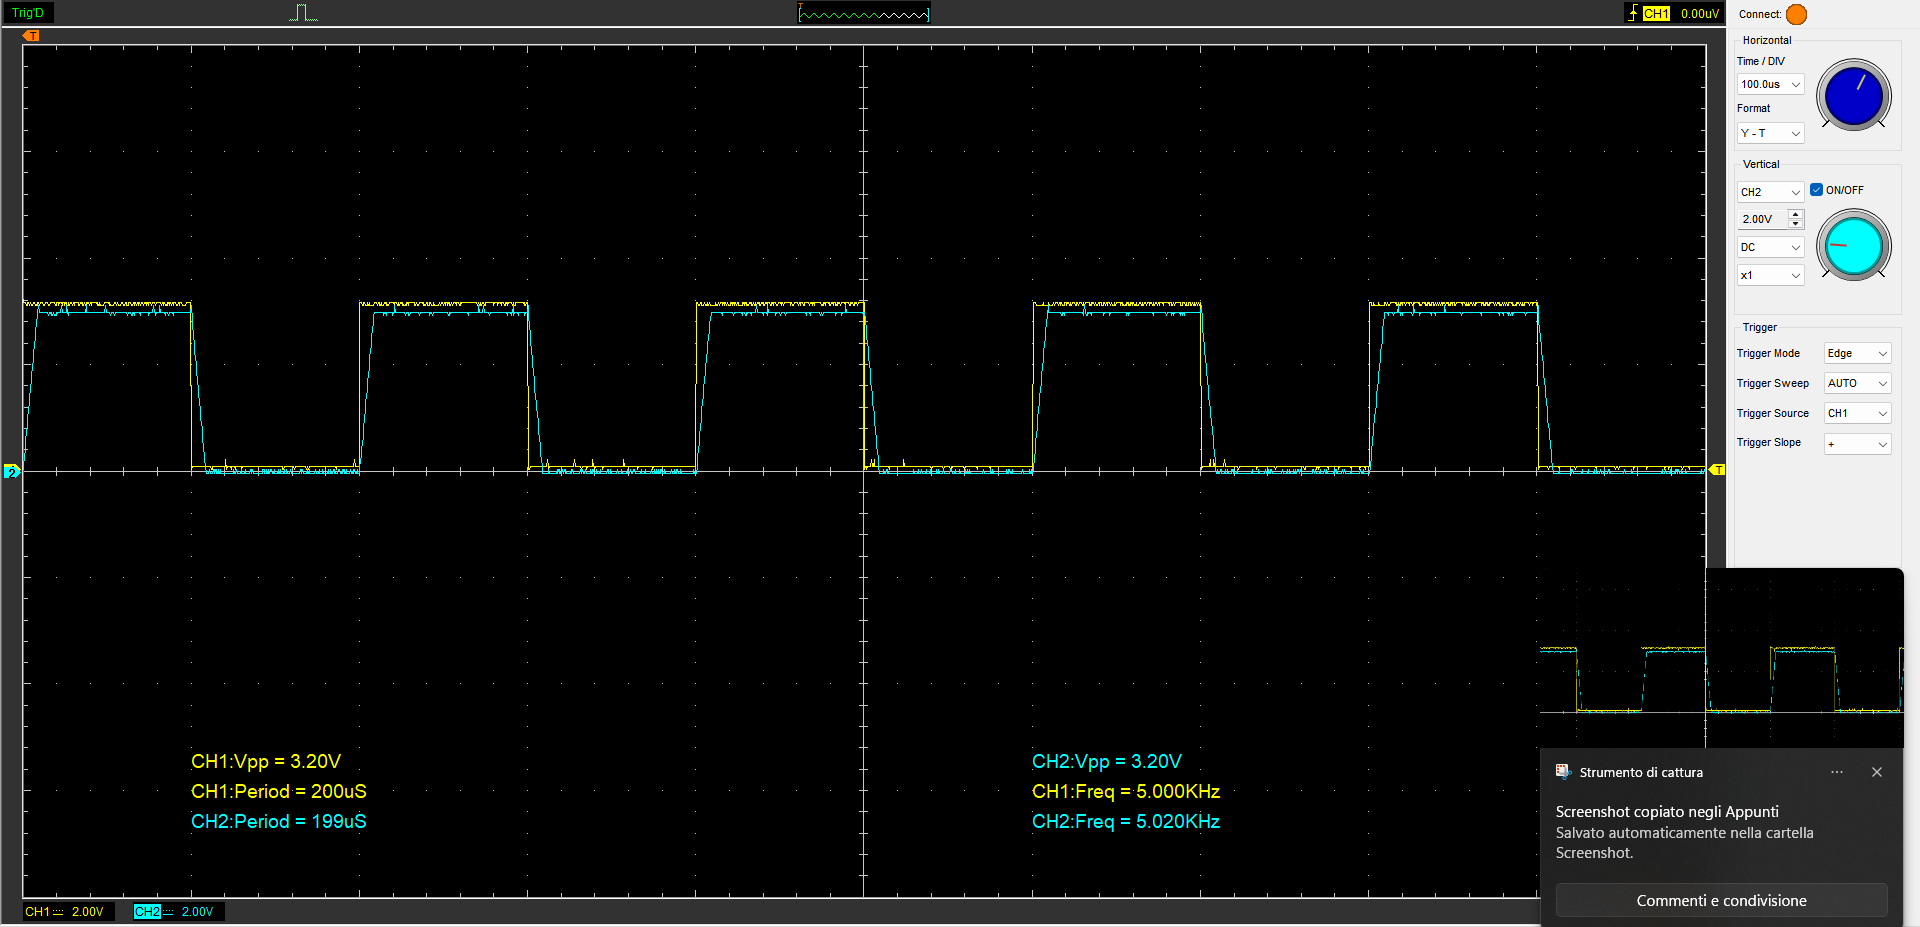
\includegraphics[width=1\textwidth]{Misc/diodo.png}
            \caption{Misurazione all'oscilloscopio del transitorio con diodo freewheeling.}
            \label{fig:transitorio_con_diodo}
        \end{figure}

        \noindent Analizzando la traccia riportata in figura \ref{fig:transitorio_con_diodo}, si nota nuovamente in giallo il segnale di pilotaggio del
        transistor e in azzurro la tensione misurata ai capi del solenoide. A differenza del caso precedente, l'inserimento del diodo di freewheeling
        abbatte completamente lo spike di sovratensione all'apertura del circuito. La tensione in eccesso viene infatti limitata (clamping) permettendo
        lo scaricamento dell'energia accumulata nell'induttore, proteggendo il circuito. Si nota che le due forme d'onda corrispondo quasi perfettamente

\newpage

\section{Risultati}

    Nella Tabella \ref{tab:risultati} sono riassunti i valori di tensione misurati dall'oscilloscopio nei due scenari analizzati.

    \begin{table}[H]
        \centering

        \begin{tabularx}{\textwidth}{|X|X|X|}
            \hline
            \textbf{Grandezza misurata} & \textbf{Senza diodo} & \textbf{Con diodo} \\ \hline
            Segnale di pilotaggio CH1 $V_{pp}$ & 3,45 V & 3,20 V \\ \hline
            Tensione ai capi del solenoide CH2 $V_{pp}$ & 8,03 V & 3,20 V \\ \hline
            Periodo del segnale & -- & 200 $\mu$s \\ \hline
            Frequenza del segnale & -- & 5,00 kHz \\ \hline
            Riduzione picco di tensione & \multicolumn{2}{X|}{\centering $\Delta V_{pp} = 8{,}03 - 3{,}20 = 4{,}83\,\text{V}\ (-60\%)$} \\ \hline
        \end{tabularx}

        \caption{Confronto delle misurazioni oscilloscopio con e senza diodo di freewheeling.}
        \label{tab:risultati}
    \end{table}

    Le misurazioni evidenziano in modo netto l'effetto del diodo di freewheeling:

    \begin{itemize}
        \item \textbf{Senza diodo di freewheeling}: la tensione ai capi del solenoide (CH2) raggiunge un valore picco-picco di 8,03 V,
            ben superiore al segnale di pilotaggio (3,45 V). Lo spike induttivo, pari a circa 4,58 V al di sopra del livello nominale, è
            riconducibile alla variazione brusca di corrente all'apertura del transistor. In sistemi alimentati a tensioni più elevate
            questo picco sarebbe proporzionalmente più pericoloso per la giunzione del transistor BDX33C ($V_{CEO,max} = 100\,\text{V}$).
        \item \textbf{Con diodo di freewheeling}: entrambi i canali mostrano la stessa ampiezza $V_{pp} = 3{,}20\,\text{V}$ e le due forme
            d'onda si sovrappongono quasi perfettamente. Lo spike è completamente soppresso: il diodo FEP16DT, entrando in conduzione diretta,
            ha offerto un percorso di scarica alla corrente induttiva residua, limitando la sovratensione a $V_F \approx 1{,}30\,\text{V}$ sopra
            l'alimentazione, in accordo con l'equazione (3).
    \end{itemize}

    \noindent Il confronto quantitativo mostra una riduzione del picco di tensione del 60\% rispetto al caso non protetto, confermando pienamente
    le previsioni teoriche e la necessità del diodo di protezione nei circuiti di pilotaggio di carichi induttivi.
    
    \newpage

\section{Conclusioni}
    In conclusione, l'esperienza di laboratorio ha permesso di verificare sperimentalmente il comportamento di un carico induttivo (il magnete solenoide)
    durante le fasi di commutazione. Tramite l'utilizzo dell'oscilloscopio è stato possibile osservare direttamente gli effetti della legge di Faraday-Lenz
    e la conseguente generazione di spike di sovratensione, che risultano essere potenzialmente distruttivi per i circuiti di pilotaggio a semiconduttore,
    come il transistor BJT impiegato nell'esperienza. \\

    \noindent Il successivo inserimento del diodo di freewheeling ha dimostrato in modo inequivocabile la sua efficacia e la sua vitale necessità: offrendo
    un percorso a bassa impedenza per il ricircolo della corrente, il diodo ha soppresso i pericolosi picchi di tensione inversa, garantendo la dissipazione
    sicura dell'energia magnetica immagazzinata nell'induttore senza recare danni al transistor. \\

    \noindent Questa prova pratica ha permesso di consolidare i concetti teorici affrontati, evidenziando l'importanza critica di adottare sempre le adeguate
    protezioni circuitali durante la progettazione di sistemi di interfacciamento tra la logica di controllo e gli attuatori elettromeccanici impiegati in ambito industriale.
\newpage

\end{document}
